\documentclass[oneside, final, 14pt]{extreport}
\usepackage[utf8]{inputenc}
\usepackage[russian]{babel}
\usepackage{vmargin}
\setpapersize{A4}
\setmarginsrb{2cm}{1cm}{1cm}{1cm}{0pt}{0mm}{0pt}{13mm}
\usepackage{indentfirst}
\usepackage{amsmath}
\usepackage{graphicx}

\begin{document}

\chapter{Физика образования и распространения звуковых волн}
\section{Природа звуковой волны}
Понятие "<звук"> может быть рассмотрено с двух принципиально различных позиций.

Звук как {\itshape физическое явление}~--- это волнообразно распространяющиеся колебания частиц упругой среды. Другими словами, звук есть результат колебательного процесса, распространяющегося в упругой среде, в частности~--- в воздушной среде.

Звук как {\itshape физиологическое явление}~--- это специфическое ощущение, вызываемое действием звуковых волн, распространяющихся в воздушной среде, на орган слуха.

Звук может распространяться только в упругой среде, т.е. в среде, которая способна восстанавливать свою первоначальную форму, искаженную (деформированную) в результате кратковременного действия на нее возмущающей силы. Упругостью сжатия и растяжения обладают как твердые тела, так и жидкие и газообразные среды. В упругой среде деформация передается последовательно от некоторой точки среды к соседней. Если, например, ударить по металлическому стержню молотком, то в месте удара образуется уплотнение металла (деформация сжатия), которое будет распространяться внутри стержня с некоторой определенной скоростью \(С\)~--- скоростью распространения звука в металле. При этом в колебательное движение придут все точки тела стержня одна за другой в направлении распространения звуковой волны. Абсолютно пластичные тела, а также частично пластичные тела, первоначальная форма которых восстанавливается только частично, практически не способны передавать звук.

Источником возникновения волнового движения (источником звука) может служить любое тело, способное совершать упругие колебания,~--- мембрана, металлическая пластина, струна, столб воздуха (в трубах) и т.д. Звуковые волны возникают благодаря упругим связям между частицами (молекулами или атомами) тела или среды, в которой находится источник звука, совершающими упругие механические колебания.

Упругие периодические механические колебания источника звука вызывают колебания близлежащих к источнику частиц упругой среды, что приводит к периодическому сжатию (сгущению) и разрежению среды в этом месте. В областях сжатия давление среды возрастает, а в областях разрежения давление понижается, т.е. возникает перепад давления в близлежащей к источнику области среды и как следствие~--- избыточное давление в этом месте.

Избыточное давление воздействует ("<толкает">) на соседние слои (элементы объема) упругой среды, которые, в свою очередь, сжимаются, и возникает избыточное давление, которое воздействует на соседний слой среды, и т.д. Приблизительно так происходит передача первоначального возмущающего импульса от источника звука в окружающей его упругой среде. Таким образом, благодаря упругим связям между молекулами и атомами среды возникает волна, которая распространяется в общем случае сначала в той среде, в которой находится источник звука (например, в воде), затем переходит в воздушную среду, где расположен слушатель, распространяется в ней и, достигая уха человека, возбуждает в нем колебания, {\itshape воспринимаемые человеком как звук}.

При совпадении направления колебаний частиц среды с направлением распространения волны возникают так называемые упругие {\itshape продольные волны}. В продольной волне частицы колеблются вперед-назад около положения устойчивого равновесия в направлении распространения волны. Продольная волна представляет собой чередование сгущений (уплотнений) и разрежений в упругой среде в направлении перемещения волны.

Упругие поперечные волны имеют место тогда, когда колебания частиц среды происходят в плоскости, перпендикулярной направлению распространения волны. Поперечные упругие волны возникают в твердых телах при сдвиге, кручении, изгибе. В этом случае возникающая деформация сдвига вызывает упругие силы, которые возбуждают упругие поперечные волны.

Не вдаваясь в сложную физику явлений, отметим лишь, что звуковые волны~--- суть продольные волны.
\section{Явления, возникающие при распространении звуковых волн}
Звук, который мы слышим,~--- это сложное явление. Звуковая волна, создающая давление на барабанную перепонку уха, на практике является результирующей звуковой волной от нескольких источников, звуковые волны которых накладываются друг на друга, отражаются, преломляются и поглощаются на своем пути. Рассмотрим эти явления.
\subsection{Интерференция}
Явление {\itshape интерференции} во времени базируется на известном принципе суперпозиции волн, смысл которого сводится к следующему: если в среде одновременно распространяется система \(n\) различных волн, то каждая из волн распространяется независимо от других. При этом результирующие скорость, смещение, ускорение каждой частицы среды равны векторным суммам соответствующих величин, обусловленных каждой из волн порознь. Если, например, наложить две синусоидальные волны \(1\) и \(2\) с различными амплитудами и длинами волн \(X_1\) и \(X_2\), то результирующая волна \(3\) получается в результате векторного суммирования смещений величин \(y_1\) и \(y_2\) обеих волн в каждой точке среды для данного момента времени \(t\) (рис. \ref{pic_interferention_01}). В этом случае результирующая волна \(3\) уже не является синусоидальной.

\begin{figure}[h]
\centering
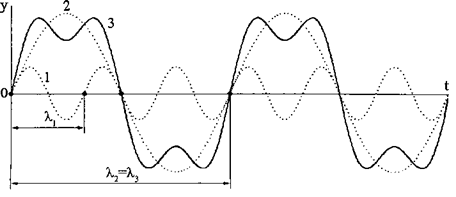
\includegraphics{pic-interferention-01}
\caption{Наложение двух волн с различными амплитудами и длинами волн}
\label{pic_interferention_01}
\end{figure}

Две волны 1 и 2 одинаковой частоты, амплитуды и фазы (т.е. одинакового начального смещения от начала координат в момент времени \(t=0\)) дают при наложении результирующую волну 3 той же частоты, но удвоенной амплитуды (рис. \ref{pic_interferention_02}).

\begin{figure}[h]
\centering
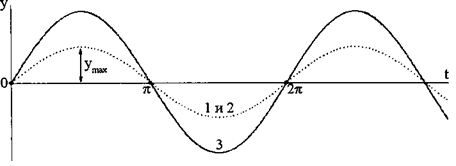
\includegraphics{pic-interferention-02}
\caption{Сумма двух колебаний одинаковой частоты, амплитуды и фазы}
\label{pic_interferention_02}
\end{figure}

Две волны 1 и 2 равной частоты, имеющие разность фаз к, нейтрализуют (гасят) друг друга при одинаковых амплитудах (т.е. результирующей волны не будет) (рис. \ref{pic_interferention_03}).

\begin{figure}[h]
\centering
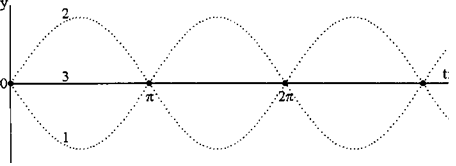
\includegraphics{pic-interferention-03}
\caption{Сумма колебаний одинаковой частоты и амплитуды и разностью фаз \(\pi\)}
\label{pic_interferention_03}
\end{figure}

Итак, звуковым волнам присуще явление интерференции, т.е. усиление колебаний в одних точках пространства и ослабление колебаний в других точках в результате наложения двух или нескольких звуковых волн, приходящих в эти точки пространства. Когда мы слышим звуки разных, но близких по величине частот (мало отличающихся частот) сразу от двух источников, к нам приходят то гребни обеих звуковых волн, то гребень одной волны и впадина другой. В результате наложения двух волн звук то усиливается, то ослабевает, пока разность фаз невелика. Этот колебательный процесс с чередующимся нарастанием и убыванием амплитуды результирующей волны называют {\itshape биением}.

На рис.\ref{pic_interferention_04} представлены два периодических гармонических колебания 1 и 2 с разными, но близкими частотами \(f_1\) и \(f_2\) и одинаковыми амплитудами \[y_{1\:max}=y_{2\:max}\].

\begin{figure}[h]
\centering
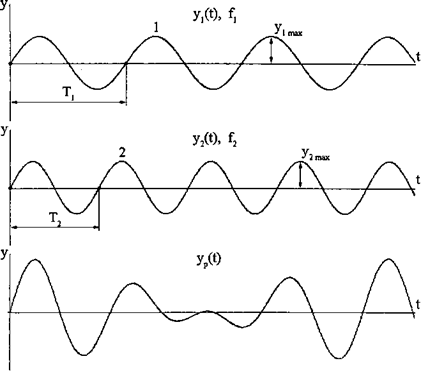
\includegraphics{pic-interferention-04}
\caption{Биение}
\label{pic_interferention_04}
\end{figure}

На этом же рисунке показано результирующее не гармоническое колебание \(y_p(t)\), являющееся суммой двух гармонических колебаний \(y_1(t)\) и \(y_2(t)\).

Как видно из рис. \ref{pic_interferention_04}, результирующее колебание \(y_p(t)\) уже не имеет постоянной амплитуды: колебания то усиливаются, то ослабевают.

При этом результирующая амплитуда \(y_{p\:max}\) периодически изменяется в пределах от \(\mid y_{1\:max}-y_{2\:max} \mid\) до \(\mid y_{1\:max}+y_{2\:max} \mid\) с частотой биения \(f_\text{б}=\mid f_2-f_1\mid\).

Биения, надо заметить, достаточно хорошо различимы на слух.

\subsection{Отражение и преломление}
Если звуковая волна, распространяющаяся в некоторой {\itshape среде 1}, достигает границы раздела этой среды с другой {\itshape средой 2}, то возникают отраженная и преломленная волны (рис. \ref{pic-reflection-01}).

\begin{figure}[h]
\centering
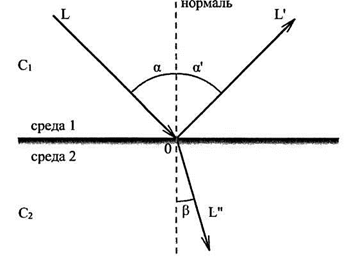
\includegraphics{pic-reflection-01}
\caption{Отражение и преломление волн на границе двух сред}
\label{pic-reflection-01}
\end{figure}

Отраженная волна распространяется от границы раздела в этой же {\itshape среде 1}, что и первичная (падающая) волна. Преломленная волна распространяется в {\itshape среде 2}. Звуковые волны подчиняются законам отражения и преломления.

Свойство отражения звуковой волны можно использовать на практике, например, для получения эффекта {\itshape эха} (отзвука). Эхо возникает при перпендикулярном отражении звуковой волны (звуковых лучей) от некоторого препятствия. При этом углы падения \(\alpha\) и отражения \(\alpha'\) будут равны \(0\). Ухо человека способно раздельно воспринять в течение секунды около 10 коротких звуков. Поэтому для возникновения эха отражающая поверхность должна быть удалена настолько, чтобы между моментом появления и моментом возврата одного звука прошло не менее \(0,1 с\). При скорости распространения звуковой волны в воздухе \(C \sim 340\)~м/с такое минимальное расстояние составляет около 17 метров.

\subsection{Поглощение и рассеяние}
Энергия звуковой волны в процессе ее распространения поглощается средой. Этот эффект называют {\itshape поглощением звуковых волн}. Существование эффекта поглощения обусловлено процессами теплообмена и межмолекулярного взаимодействия в среде, точнее~--- внутренним трением и теплопроводностью. Под энергией звуковой волны следует понимать кинетическую и потенциальную энергию частиц (атомов и молекул) сжимаемого элемента объема упругой среды в направлении распространения звуковой волны.

Степень поглощения звуковой энергии при распространении звуковой волны в жидкостях и газах зависит, с одной стороны, от свойств среды, а с другой~--- от частоты звуковых колебаний. Чем выше частота звуковых колебаний, тем больше хаотическая молекулярная скорость молекул в элементе сжимаемого объема, тем большее молекулярное рассеяние претерпевает на своем пути звуковая волна и тем на меньшее расстояние передаются звуковые колебания.

{\itshape Рассеяние звука} возникает в результате взаимодействия звуковой волны со встречающимися на ее пути многочисленными препятствиями (встречные потоки воздуха, завихрения, ветер). В результате столкновения с этими препятствиями звуковая волна как бы "<рассыпается"> на множество волн, которые распространяются во всевозможных направлениях.

\subsection{Волновое движение в замкнутом объеме}
С отражением и поглощением звука тесно связано явление волнового движения в замкнутом объеме, когда волны отражаются то от одной, то от другой стенки помещения (потолка, пола). Отражения звуковых колебаний могут сильно влиять на конечное восприятие звука: они могут изменять окраску звука, насыщенность, глубину. Так, звук, идущий от источника, расположенного в закрытом помещении, многократно ударяясь и отражаясь от стен помещения, воспринимается слушателем как звук, сопровождающийся специфическим гулом. Такой гул называется {\itshape реверберацией} (от лат. "<reverbero">~--- "<отбрасываю">). Появление реверберации связано с тем, что звуковая волна, исходящая от источника звука, на пути к слушателю накладывается на многократно отраженные от стен и потому сдвинутые во времени копии самой себя (рис. \ref{pic-reverberation-01}).

\begin{figure}[h]
\centering
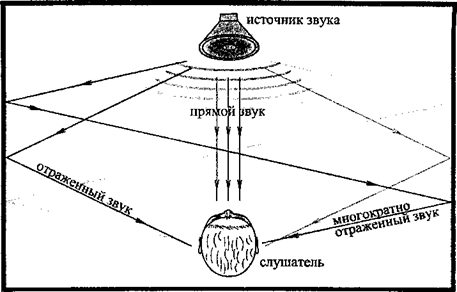
\includegraphics{pic-reverberation-01}
\caption{Диаграмма прохождения звуковой волны от источника к слушателю в закрытом помещении}
\label{pic-reverberation-01}
\end{figure}

Отражения звука принято делить на {\itshape ранние отражения} и собственно {\itshape реверберацию}. Ранними отражениями называют повторения прямого звука, пришедшие к слушателю в течение первых 50 мс. Остальные отражения приходят к слушателю многократно наложенными друг на друга и составляют тот самый гул реверберации. Ранние отражения являются особо важными для человеческого слуха в виду эффекта, известного как эффект Хааса. {\itshape Эффект Хааса} заключается в том, что слуховая система человека определяет направление прихода звука по направлению прихода прямого звука, а не по его ранним отражениям. Ввиду разницы в физических свойствах различных материалов их отражающая способность разная. По этой причине, а также ввиду различий в конфигурации помещений, время, состав реверберации и количество ранних отражений в разных помещениях может сильно отличаться. Принято считать, что количество, время и сила ранних отражений несут информацию о геометрии помещения, а состав реверберации~--- о материале поверхностей.

\subsection{Дифракция}
Очень важное свойство звуковых волн~--- способность огибать малые препятствия. Это явление называют {\itshape дифракцией звуковых волн}. Суть этого явления заключается в том, что плоская звуковая волна возбуждает у краев препятствия элементарные волны, сходящиеся позади препятствия. Таким образом волна проникает в область геометрической тени. Степень огибания зависит от соотношения между длиной приходящей звуковой волны и размером стоящего на ее пути препятствия (или отверстия). Если размер препятствия намного больше длины волны, то звуковая волна отражается от такого препятствия. Если же размеры препятствия сопоставимы с длиной волны или меньше ее, то звуковая волна дифрагирует.

С дифракцией звука мы сталкиваемся в повседневной жизни постоянно. Если бы дифракции звука не существовало, то мы бы не слышали, например, музыку, звучащую за углом дома, не смогли бы слышать разговор за закрытой дверью и т.д.

\subsection{Вынужденные и собственные колебания, резонанс}
Рассмотрим еще одно явление, связанное с распространением звука в воздушной среде,~--- явление звукового резонанса.

В общем случае, {\itshape резонанс}~--- это эффект резкого возрастания амплитуды вынужденных колебаний какой-то упругой системы при близком приближении или полном совпадении частоты вынужденных колебаний с собственной частотой этой системы.

Вынужденные колебания системы вызываются действием на нее периодических внешних возмущающих сил. Вынужденные периодические колебания в упругой звуковой среде могут создавать любые тела, совершающие периодические механические колебания (мембрана, диффузор, струна и т.д.).

{\itshape Собственная частота} некоторой системы~--- это частота свободного колебания этой системы. {\itshape Свободными колебаниями} называются такие колебания, которые возникают в упругой системе в результате какого-либо одноразового начального отклонения системы от состояния устойчивого равновесия.

Например, гитарная струна при ударе по ней начинает колебаться довольно продолжительное время, т.е. совершать свободные затухающие колебания. При этом воздушная среда вокруг колеблющейся струны начинает колебаться с частотой струны (собственно, благодаря этому мы и слышим звук гитары), т.е. совершать {\itshape вынужденные колебания с частотой свободных колебаний} струны.

Явление резонанса следует отличать от {\itshape эффекта усиления вынужденных колебаний}, возникающих при несовпадении частоты возмущающей силы и собственной частоты. Например, если поставить звучащий камертон на стол, то доска стола приходит в вынужденные колебания и звук усиливается, но это объясняется простым увеличением площади колеблющейся поверхности, а не совпадением частот.

Резонанс звука может быть желательным и нежелательным явлением. Например, телефонные и микрофонные мембраны могут колебаться на различных вынуждающих частотах, но при этом резонанса стараются избежать (резонанс должен лежать вне желаемой области частот, иначе резонансные частоты будут воспроизводиться чрезмерно громко). А вот в акустике при прослушивании шумов, создаваемых различными объектами, при настройке различной радиоаппаратуры, при выборе нужной частоты в радиоприемнике и т.д. явление резонанса создается специально.

\subsection{Эффект Доплера}
Рассмотрим еще одно явление, связанное с распространением звуковых волн~--- эффект Доплера. До сих пор предполагалось, что источник звуковой волны и ее приемник неподвижны по отношению к среде, в которой происходит распространение звуковых колебаний. Своеобразные эффекты, проявляющиеся при взаимном перемещении относительно неподвижной среды источника и приемника звуковых волн, впервые обнаружил Доплер в 1842 году. Он обратил внимание на то обстоятельство, что при перемещении только лишь источника или только лишь приемника или при одновременном перемещении и источника, и приемника относительно среды, в которой распространяется звуковая волна, частота колебаний, воспринимаемая приемником, изменяется. Зависимость частоты колебаний, воспринимаемых приемником, от скоростей движения источника волн и приемника по отношению к среде, в которой распространяется звуковая волна, была названа эффектом Доплера.

Наглядно проиллюстрировать эффект Доплера можно с помощью простейшего примера, представленного на рис. \ref{pic-dopler-01}.

\begin{figure}[h]
\centering
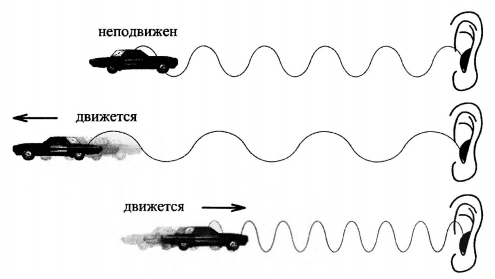
\includegraphics{pic-dopler-01}
\caption{Иллюстрация Эффекта Доплера}
\label{pic-dopler-01}
\end{figure}

Наверное, все когда-нибудь замечали, что звук мотора приближающегося автомобиля кажется нарастающим по высоте, в то время как высота звука, издаваемого мотором удаляющегося автомобиля, наоборот,~--- падающей. Этот пример и является простейшей демонстрацией эффекта Доплера.

Эффект Доплера используется в самых различных отраслях человеческой деятельности для измерения скорости объектов на расстоянии. Так, например, в медицине с помощью ультразвука (высокочастотных звуковых колебаний) измеряют скорость прохождения крови по сосудам. Принцип действия устройства, осуществляющего такое измерение, заключается в следующем: источник ультразвука испускает ультразвуковую волну, которая, встречаясь в крови с эритроцитом, ударяется о него и отражается в обратном направлении, после чего улавливается датчиком. По разнице длин выпущенной и пришедшей волн можно определить скорость движения эритроцитов, а значит, и скорость прохождения крови. На аналогичном принципе действия основаны и самые различные средства радиолокации.

\section{Математическое представление звуковой волны}
\subsection{Уравнение звуковой волны}
Звуковые (или любые другие) колебания называются {\itshape периодическими}, если значения физических величин, изменяющихся в процессе колебаний, повторяются через равные промежутки времени, а именно через период колебания \(T\).

За это время совершается одно полное колебание. В непериодических звуковых колебаниях отсутствует указанное выше понятие периода, т.е. отсутствует периодическая повторяемость физических величин, изменяющихся в процессе колебания.

{\itshape Частотой колебаний} называют количество полных колебаний в секунду. За единицу измерения частоты принят 1 герц (Гц). 1 герц соответствует одному полному колебанию, происходящему за одну секунду.

Примером периодического звукового колебания может служить приятно воспринимаемый на слух музыкальный звук. К непериодическим звуковым колебаниям относятся различные шумы и многие другие природные звуки. Простейшим видом периодических колебаний являются синусоидальные (или гармонические) колебания, которые описываются математически с помощью следующего уравнения:
\[y(t)=A\sin(\omega t+\varphi)\]
где
\begin{itemize}
\item \(y(t)\)~--- условное обозначение физической величины, которая изменяется в функции времени по синусоидальному закону;
\item \(A\)~--- амплитуда колебания, т.е. максимальное значение функции \(у(t)\);
\item \(\omega=2\pi f=\frac{2\pi}{T}\)~--- угловая (циклическая) частота колебаний;
\item \(f\)~--- частота колебаний;
\item \(\varphi\)~--- начальная фаза колебаний, т.е. сдвиг по оси абсцисс от начала координат функции \(y(t)\) в момент времени \(t=0\).
\end{itemize}

Под понятием {\itshape спектра звукового сигнала} (звуковой волны) следует понимать совокупность составляющих синусоидальных звуковых волн, в результате наложения которых получается исходная результирующая звуковая волна. Совокупность (набор) значений амплитуд и частот составляющих синусоидальных волн называется соответственно спектром амплитуд и спектром частот.

Рассмотрим колебания воздушной среды, в которой источником возмущения является камертон. Как известно, колеблющийся (звучащий) камертон возбуждает в воздушной среде почти чистую синусоидальную продольную звуковую волну (такую волну называют простым или чистым тоном). Пусть частица воздушной среды, находящаяся в начале отсчета пространства (т.е. частица, находящаяся возле колеблющейся пластины камертона в
точке пространства \(х=0\)) в момент времени \(t=0\) начинает колебательное движение в направлении распространения продольной звуковой волны по закону:

\[y(t)=A\sin(\omega t) = A\sin(\frac{2\pi}{T}t),\]
где \(y(t)\)~--- величина смещения по оси ординат от нулевого значения \((x=0)\) в зависимости от времени \(t\). Эта частица, как и все последующие частицы (точки) воздушной среды, придет в колебательное движение около своего положения равновесия в направлении распространения звуковой волны по синусоидальному закону.

Последующие частицы будут начинать свои колебания на \(\Delta t\) секунд позже в зависимости от удаленности частицы от начала координат по оси абсцисс (расстояние \(х\)). Этот промежуток времени можно определить как
\[\Delta t=\frac{x}{C},\]
где \(C\)~---  скорость распространения звуковой волны в воздушной среде. Тогда величину смещения у для любой точки среды в направлении распространения звуковой волны можно выразить как
\[y(t)=A\sin[\omega (t-\Delta t)] = A\sin[\omega(t-\frac{x}{C})],\]

Учитывая, что \(C=\lambda f=\frac{\lambda}{T}\) и \(\Delta t=\frac{x}{C}\), это уравнение можно записать как

\[y(t) = A\sin[2\pi(\frac{t}{T}-\frac{\Delta t}{T})] = A\sin[2\pi(\frac{t}{T}-\frac{x}{CT})]=A\sin[2\pi(\frac{t}{T}-\frac{x}{\lambda})]\]
где \(\lambda\)~--- длина звуковой волны.

Полученное уравнение называется {\itshape уравнением звуковой волны} и описывает колебания всех частиц (точек) звуковой волны, расположенных на любых расстояниях \(х\) по отношению к начальной точке.

\subsection{Способы графического отображения звуковых сигналов}
В предыдущих разделах при представлении графика звуковой волны (звука) в функции времени, мы "<по умолчанию"> подразумевали реальную упрощенную звуковую волну (звук), преобразованную с помощью соответствующей аппаратуры в электрический сигнал, изменяющийся во времени идентично звуковой волне (т.е. моделирующий ее форму) и выведенный либо на экран осциллографа или монитора компьютера, либо с помощью различных самописцев на бумагу и т.д.

Способ графического отображения звукового сигнала в виде значений его уровня (амплитуды) во времени называют {\itshape амплитудно-временным}, а сам график, отображающий зависимость амплитуды текущего звукового сигнала в функции времени,~--- осциллограммой или сигналограммой. Из английского языка в русский было заимствовано понятие "<{\itshape волновая форма}">, которая является синонимом сигналограммы. В качестве примера на рис. \ref{pic-waveform-01} представлена сигналограмма записи человеческой речи (произнесенная вслух фраза "<раз-два-[пауза]-три-четыре">), записанной с помощью компьютера.

\begin{figure}[h]
\centering
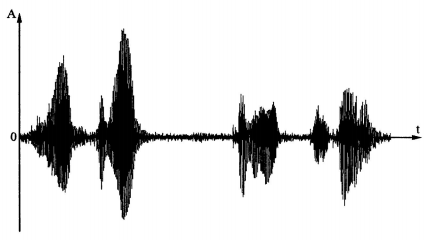
\includegraphics{pic-waveform-01}
\caption{Сигналограмма записи человеческой речи}
\label{pic-waveform-01}
\end{figure}

Если очертить сигналограмму сверху и снизу таким образом, что изображенные на ней колебания окажутся "<вписанными"> между очерчивающими их линиями, то в результате получится график амплитудной огибающей сигнала. На рис. \ref{pic-waveform-02} показан график амплитудной огибающей сигнала, представленного на рис. \ref{pic-waveform-01}.

По форме амплитудной огибающей (как и по форме самой сигналограммы) можно судить о характере изменения интенсивности звука на всей его протяженности и тем самым визуально определять, например, где находятся промежутки между словами (на рисунке такой промежуток обозначен {\itshape в}) и паузы (промежуток {\itshape б}), а где~--- громкие звуки (промежуток {\itshape а}).

\begin{figure}[h]
\centering
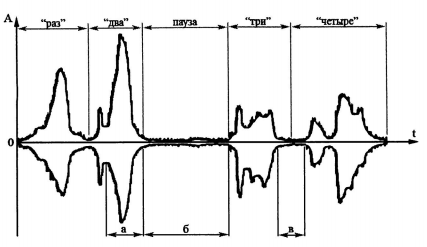
\includegraphics{pic-waveform-02}
\caption{График амплитудной огибающей}
\label{pic-waveform-02}
\end{figure}

Обобщенная форма амплитудной огибающей большинства существующих в природе одиночных звуков может быть представлена в виде графика, показанного
на рис. \ref{pic-waveform-03}.

\begin{figure}[h]
\centering
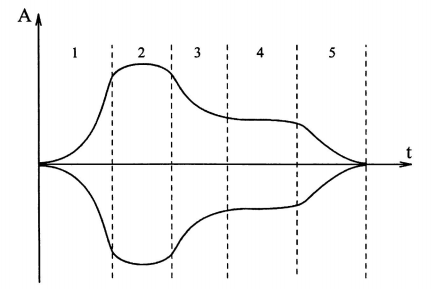
\includegraphics{pic-waveform-03}
\caption{График типичной амплитудной огибающей реального одиночного звукового сигнала}
\label{pic-waveform-03}
\end{figure}

Эта форма подразумевает условное деление огибающей амплитуды на пять частей, т.е. пять фаз развития звуковой волны.
\begin{enumerate}
\item Атака, подъем (от англ. "<attack">).
\item Стабилизация (от англ. "<hold">).
\item Спад (от англ. "<decay">).
\item Удержание (от англ. "<sustain">).
\item Затухание (от англ. "<release">).
\end{enumerate}

В отношении фазы удержания нужно отметить, что она различима только в тех звуках, которые вызваны каким-то продолжительным во времени воздействием. Звуки, вызванные кратковременным, почти мгновенным воздействием, имеют почти нулевую фазу удержания.

На рис. \ref{pic-waveform-04} представлена сигналограмма короткого звука виолончели, из которой видно, что очертания этой сигналограммы очень схожи с типичной амплитудной огибающей, рассмотренной выше, т.е. налицо все пять фаз развития звуковой волны.

\begin{figure}[h]
\centering
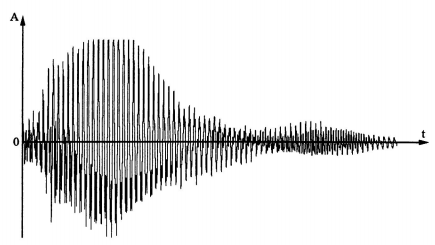
\includegraphics{pic-waveform-04}
\caption{Сигналограмма короткого звука виолончели}
\label{pic-waveform-04}
\end{figure}

Звук большинства духовых инструментов также имеет амплитудную огибающую со всеми пятью перечисленными фазами. В то же время большинство немузыкальных звуков, как, например, звук щелчка пальцами, имеют очень непродолжительную фазу стабилизации и почти нулевую фазу удержания.

Второй способ графического представления звуковых сигналов заключается в его отображении в виде амплитудно-частотной зависимости, т.е. в виде графика амплитудно-частотного спектра, на котором по оси абсцисс откладываются частоты составляющих спектра, а по оси ординат~--- амплитуды соответствующих частотных составляющих.

В качестве примера на рис. \ref{pic-specter-01} приведен график спектра реального аудиосигнала (речи), сигналограмма которого показана на рис. \ref{pic-waveform-01}. На приведенном графике амплитуды спектральных составляющих можно соединить кривой, которая называется амплитудной огибающей спектра сигнала или просто спектральной огибающей.

\begin{figure}[h]
\centering
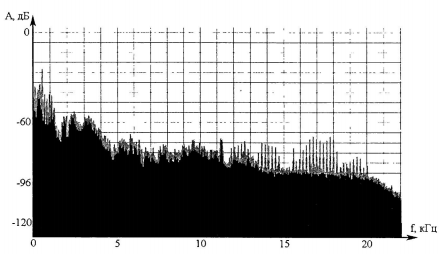
\includegraphics{pic-specter-01}
\caption{Спектр записи речи}
\label{pic-specter-01}
\end{figure}

Разложение реального звукового сигнала в спектр целиком на практике применяется редко; реальные звуковые сигналы на практике чаще всего анализируют поблочно. В этом случае спектр всего сигнала представляет собой уже не один амплитудно-частотный график, а целую серию таких графиков (каждому блоку анализируемого сигнала соответствует отдельная спектральная картинка). Серию таких спектров можно отобразить в виде так называемой спектрограммы.

{\itshape Спектрограмма}~--- это псевдо-трехмерный график в прямоугольной системе координат, на котором по оси \(X\) откладывается время, по оси \(Y\)~--- частота, а амплитуды частотных составляющих изображаются в соответствующих точках графика насыщенностью цвета.

На рис. \ref{pic-specter-02} в качестве примера показана спектрограмма аудиозаписи речи (сигналограмма этого звукового сигнала представлена на рис. \ref{pic-waveform-01}).

\begin{figure}[h]
\centering
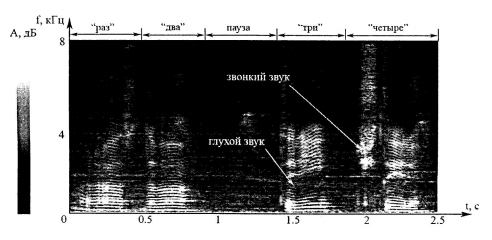
\includegraphics{pic-specter-02}
\caption{Спектрограмма записи речи}
\label{pic-specter-02}
\end{figure}

Спектрограмма~--- это очень мощный графический инструмент спектрального анализа, поскольку она обеспечивает наилучшее визуальное представление спектра и позволяет в подробностях анализировать динамику развития сигнала.

Нередко встречается также непосредственно трехмерное представление спектра сигнала в виде трехмерной спектрограммы. Способ отображения спектра в случае трехмерной спектрограммы фактически аналогичен способу, примененному в обыкновенной спектрограмме, с той лишь разницей, что амплитуды частотных составляющих изображаются на трехмерной спектрограмме не интенсивностью цвета (точнее, не только интенсивностью цвета), а путем откладывания величины амплитуды по третьей координатной оси \(Z\). На рис. \ref{pic-specter-03} представлена трехмерная спектрограмма звукового сигнала с записью речи (его сигналограмма показана на рис. \ref{pic-waveform-01})

\begin{figure}[h]
\centering
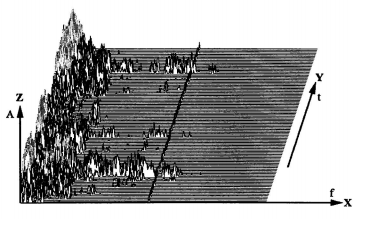
\includegraphics{pic-specter-03}
\caption{Трехмерная спектрограмма звукового сигнала с записью речи}
\label{pic-specter-03}
\end{figure}

\subsection{Гармонический анализ реальных звуковых сигналов}
Суть {\itshape гармонического анализа} сводится к следующему: любое периодическое колебание с частотой \(\omega\) можно представить в виде суммы гармонических колебаний, и наоборот, зная параметры отдельных гармоник (амплитуду, частоту и начальную фазу), можно с помощью их тригонометрического суммирования получить (или приближенно смоделировать) результирующее колебание.

Другими словами, любую сложную периодическую функцию можно разложить в тригонометрический гармонический ряд (называемый рядом Фурье) и анализировать эту функцию при помощи гармонического анализа, т.е. анализа гармоник, составляющих эту результирующую функцию. В общем случае ряд Фурье для временной периодической функции \(y(t)\) выглядит следующим образом:

\[ y(t) \approx \frac{a_0}{2} + \sum\limits_{v=1}^{\infty}(a_v\cos(v\omega t) + b_v\sin(v\omega t)),\]

Сумма гармонических колебаний с периодами \(T_1, \frac{1}{2}T_1, \frac{1}{3}T_1,...,\frac{1}{v}T_1\), где \(\frac{1}{v}T_1=T_v\)~--- период \(v\)-ой гармоники дает результирующее колебание с периодом \(T_1\). Это правило относится и к частотам \(\omega\), а именно: сумма любого числа гармонических колебаний с частотами, кратными \(\omega_1\), т.е. \(\omega_1, 2\omega_1,3\omega_1,...,v\omega_1\) дает результирующее колебание с частотой \(\omega_1\).

Угловая частота \(\omega_1=2\pi f_1\) называется {\itshape основной гармоникой} или {\itshape основной частотой}.
Частоты \(\omega_2=2\omega_1, \omega_3=3\omega_1,...,\omega_v=v\omega_1\)~--- это {\itshape обертоны} или просто {\itshape гармоники} (говорят, "<вторая гармоника">, "<третья гармоника"> и т.д.).

Представление функции \(y(t)\) в виде суммы гармонических колебаний называется {\itshape разложением функции в спектр}. Под спектром функции следует понимать данные о частотах ({\itshape частотный спектр}), амплитудах ({\itshape амплитудный спектр})и начальных фазах ({\itshape спектр начальных фаз}).

Спектр звукового сигнала является одним из важнейших инструментов анализа и обработки звука.
Качество музыкального (и немузыкального) звука зависит от состава его частотного спектра и правильного выбора пропорций частот, входящих в этот спектр. Другими словами, упомянутое "<качество"> определяется, во-первых, относительным количеством различных гармоник в спектре звука, а во-вторых, относительными значениями коэффициентов
ряда Фурье, которые указывают, с "<каким весом"> каждая гармоника входит в общее колебание (т.е. в результирующую функцию).

Считается, что из неэлектронных средств и устройств только камертон может обеспечить практически чистый
тон. Все музыкальные и немузыкальные звуки, не говоря уже о звуковых шумах, имеют широкий частотный спектр. Даже один и тот же музыкальный тон, взятый на разных инструментах, будет иметь одну и ту же основную частоту, но разные
частотные спектры, т.е. разный {\itshape тембр}.

{\itshape Тембровая окраска звука} определяется распределением интенсивности обертонов (высших гармоник). Всем хорошо известно, что чем сложнее спектр, тем богаче тембр звука в музыкальном отношении.

Сегодня существует много разнообразных электронных музыкальных инструментов, в которых, благодаря использованию осцилляторов (устройств, генерирующих чистые гармонические колебания), усилителей звука и других специальных
преобразователей, смешивают гармоники в любой желаемой пропорции и тем самым создают звуки различного качества (синтез звука).

Гармонический анализ различных шумов имеет большое практическое значение (особенно это касается производства и специальной техники, где шумы просто недопустимы, например подводные лодки, авиация и т.д.), так как по частотному и амплитудному спектрам устанавливают причины шума, чтобы затем устранить их полностью или ослабить до допустимых норм; анализ шумовых характеристик приборов и механизмов позволяет обнаруживать и устранять неполадки в них
и т.д.

\subsection{Гармонический анализ реальных звуковых сигналов}
Реальные звуковые сигналы являются сложными и их практически невозможно описать в виде какой-либо математической
функции или с помощью эмпирической аналитической зависимости. Анализируемый реальный звуковой сигнал является, как правило, "<вырванным из контекста">, т.е. фрагментом некоторой длины, являющимся частью общего, возможно, очень
продолжительного, звукового материала.

Таким образом, фрагментальный спектральный анализ может осуществляться как по чисто объективным причинам
(в частности, из-за невозможности и нецелесообразности спектральной обработки целиком продолжительных звуковых сигналов), так и при необходимости оценки шумовых, тембровых и других характеристик в отдельных фрагментах звукового материала.

Реальный звуковой сигнал может быть графически представлен в виде сигналограммы и спектрограммы. Поскольку сегодня большинство операций обработки и анализа сигналов проводят с использованием цифровой аппаратуры, во всех перечисленных способах графического представления сигнал в большинстве случаев описывается его дискретными параметрами: дискретной амплитудой, дискретной частотой и дискретным временем, что объясняется
способом регистрации сигнала.

Для того чтобы реальную звуковую волну можно было анализировать с помощью гармонического анализа с применением цифровой вычислительной техники, волну представляют в некотором дискретном виде, т.е. в виде ряда чисел, тем или иным образом описывающих ее форму.

Для получения частотного спектра сигнала, описанного его дискретными значениями, применяют {\itshape дискретное преобразование Фурье}, или {\itshape ДПФ} (Discrete Fourier Transform~--- DFT),~--- специально созданную разновидность преобразования Фурье, предназначенную для спектрального разложения дискретных сигналов.

Чтобы сделать вычисления ДПФ в цифровой вычислительной технике более эффективными, был создан алгоритм, названный быстрым преобразованием Фурье, или БПФ (Fast Fourier Transform - FFT).

С использованием ДПФ звуковой сигнал, описанный дискретными численными значениями, может быть представлен в виде амплитудно-частотного спектра. Любой, даже самый сложный по форме сигнал (например, звук голоса человека),
можно представить суммой простейших синусоидальных колебаний определенных частот и амплитуд. Помимо специальной техники разложения в спектр сигналов, заданных именно дискретными значениями (а не аналитическим выражением),
в основе ДПФ лежит идея, аналогичная идее спектрального разложения непериодических функций: произвольный (непериодический) сигнал, точнее~--- анализируемый фрагмент сигнала, представляется как один период некоторого бесконечного периодического сигнала, который и раскладывается в частотный спектр.

Рассмотрим пример такого спектрального разложения. Возьмем сложную реальную звуковую волну, заданную дискретными значениями ее амплитуды в функции времени, и проследим, как на практике она раскладывается в тригонометрическую сумму синусоидальных составляющих (ряд Фурье) и анализируется.

На рис. \ref{pic-specter-04} представлен фрагмент сигналограммы реальной звуковой волны~--- фрагмент музыкальной аудиозаписи продолжительностью 0,25 с (на графике по оси абсцисс откладывается время, а по оси ординат~--- дискретные значения амплитуд \(А\), которые на сигналограмме сливаются в сплошную линию).

Будем считать, что представленный на сигналограмме звуковой сигнал является рабочим фрагментом, выбранным для проведения спектрального анализа. Теперь с помощью ДПФ (БПФ) проведем спектральное разложение представленного фрагмента звукового сигнала. При спектральном разложении обрабатываемый фрагмент представляется в виде одного периода некоторого бесконечного периодического звукового сигнала, полученного путем периодического продолжения анализируемого фрагмента.

\begin{figure}
\centering
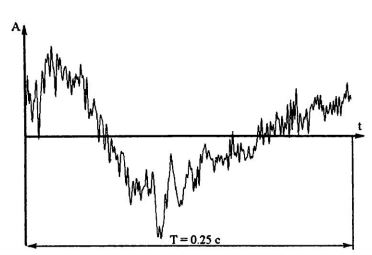
\includegraphics{pic-specter-04}
\caption{Сигналограмма фрагмента музыкальной аудиозаписи продолжительностью 0.25с}
\label{pic-specter-04}
\end{figure}

ДПФ раскладывает анализируемый фрагмент в амплитудно-частотный спектр и дает на выходе в четкой последовательности набор гармоник и соответствующие им значения амплитуд. Из полученного набора гармоник можно составить частичные
суммы с тем, чтобы наглядно наблюдать за приближением гармонического ряда к исходному сигналу.
Посмотрим, как соотносится первая частичная сумма \(S(x,1)\) с анализируемым фрагментом аудиосигнала (рис. \ref{pic-specter-05}).

Частичная сумма \(S(x,1)\) представляет собой основную гармонику спектра. Как видно из рисунка, \(S(x,1)\) является синусоидой, лишь приблизительно повторяющей очертания исходного сигнала. Теперь возьмем вторую частичную сумму \(S(x,2)\), состоящую из первых двух гармоник спектра (рис. \ref{pic-specter-06}).

Как видно из рис. \ref{pic-specter-06}, и в этом случае \(S(x,2)\) лишь приблизительно повторяет очертания исходного сигнала. На рис. \ref{pic-specter-07} и \ref{pic-specter-08} представлены частичные суммы \(S(x,15)\) и \(S(x,40)\) соответственно.

Из приведенных графиков видно, что чем большее число гармоник мы суммируем, тем более точное приближение исходного сигнала мы получаем. В данном приближении при суммировании 130 членов ряда частичная сумма \(S(x,130)\)
приобретает очертания оригинального сигнала с неотличимыми на глаз различиями.

Рассмотренный пример позволяет нам еще раз убедиться в том, что низкочастотные составляющие спектра придают суммирующей волне общую правильность формы, тогда как высокочастотные составляющие уточняют форму
волны, привнося в нее мелкие детали исходного сигнала.

Для полноты картины на рис. \ref{pic-specter-09} представлен график амплитудно-частотного спектра рассмотренного аудиосигнала.

\begin{figure}
\centering
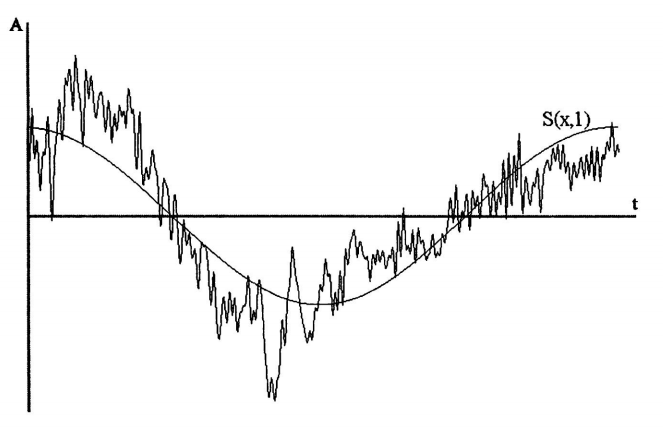
\includegraphics{pic-specter-05}
\caption{Сигналограмма аудиофрагмента и график частичной суммы \(S(x,1)\)}
\label{pic-specter-05}
\end{figure}

\begin{figure}
\centering
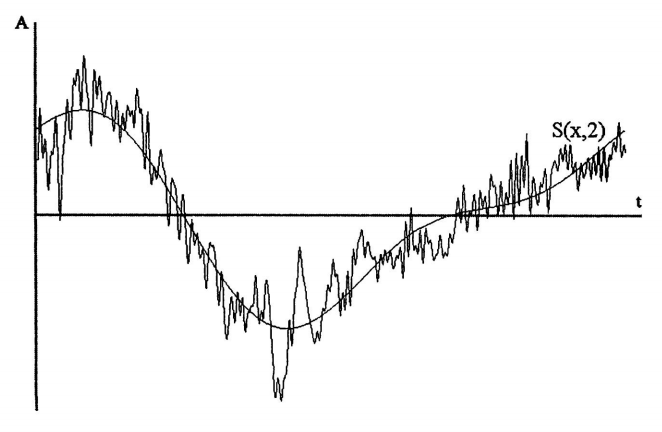
\includegraphics{pic-specter-06}
\caption{Сигналограмма аудиофрагмента и график частичной суммы \(S(x,2)\)}
\label{pic-specter-06}
\end{figure}

\begin{figure}
\centering
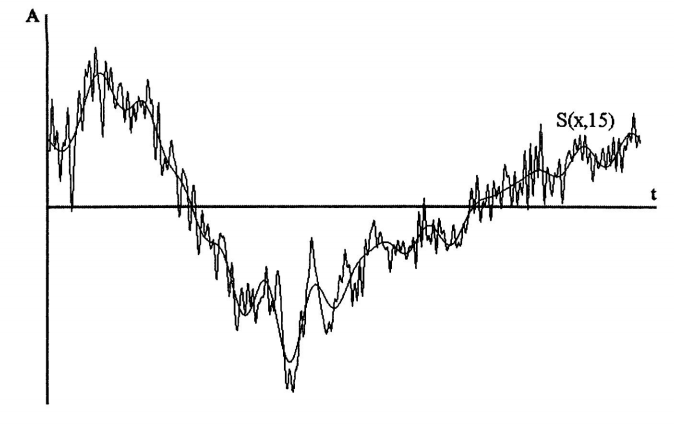
\includegraphics{pic-specter-07}
\caption{Сигналограмма аудиофрагмента и график частичной суммы \(S(x,15)\)}
\label{pic-specter-07}
\end{figure}

\begin{figure}
\centering
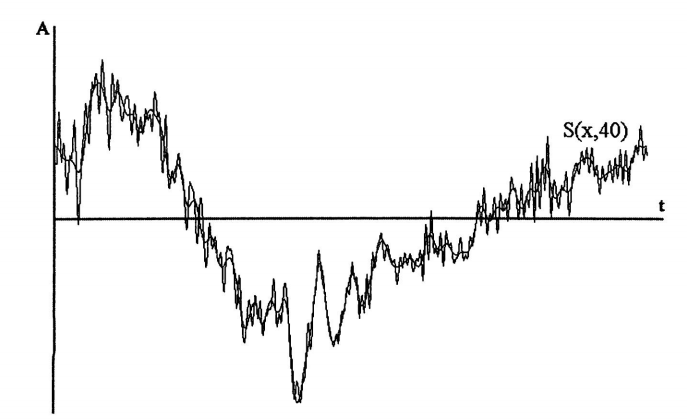
\includegraphics{pic-specter-08}
\caption{Сигналограмма аудиофрагмента и график частичной суммы \(S(x,40)\)}
\label{pic-specter-08}
\end{figure}

\begin{figure}
\centering
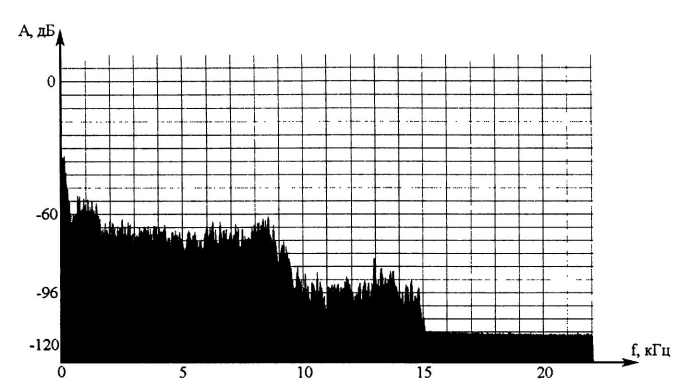
\includegraphics{pic-specter-09}
\caption{Полный спектр анализируемого аудиофрагмента}
\label{pic-specter-09}
\end{figure}

\subsection{Блочный спектральный анализ}
Идея блочного спектрального анализа заключается в проведении гармонического анализа реального звукового сигнала таким образом, который позволил бы видеть динамику изменения частотного и амплитудного спектров анализируемого сигнала во времени. Другими словами, идея заключается в осуществлении спектрального анализа так, чтобы можно было увязать, грубо говоря, звук в какой-то момент времени и соответствующий этому моменту времени спектр звуковой волны. До этого же речь шла как бы о "<статическом анализе">, т.е. для какой-то функции (или фрагмента) определялся частотный и амплитудный спектры, но при этом мы не могли даже приблизительно ответить на вопрос "<Какая частота или диапазон частот соответствует звуковому сигналу в тот или иной момент времени?">.

Чтобы конкретизировать идею блочного спектрального анализа, рассмотрим следующий реальный пример.

Предположим, что перед нами стоит задача проанализировать аудиофрагмент длительностью 50 секунд некоторой фонограммы с целью выявления каких-то спектральных характеристик на определенных интересующих нас временных участках этого фрагмента. Если мы "<по привычке"> разложим этот фрагмент фонограммы целиком в амплитудно-частотный спектр, то в результате получим статичную картинку спектра (подобную представленной на рис. \ref{pic-specter-09}), которая даст нам четкое представление о том, какие частоты и с какими амплитудами присутствуют в рассматриваемом звуковом фрагменте длительностью 50 секунд. А теперь возникает вопрос "<Что же делать дальше с полученной спектральной информацией?">.
Ведь, с одной стороны, нам приблизительно известны временные координаты интересующих нас участков пятидесятисекундного фрагмента фонограммы, но, с другой стороны, мы не можем привязать полученный амплитудно-частотный спектр к этим отдельным участкам. Таким образом, спектральный анализ всего пя-
тидесятисекундного фрагмента фонограммы целиком не отражает динамику развития звуковых колебаний во времени внутри этого фрагмента; получаемая спектральная картина является общей для всего пятидесятисекундного фрагмента и характеризует весь фрагмент целиком, но не отдельные его части. Понимание этого факта является очень важным и принципиальным. Выражаясь математическим
языком, преобразование Фурье переносит анализируемую величину из амплитудно-временного пространства в амплитудно-частотное (рис. \ref{pic-specter-10}).

\begin{figure}[h]
\centering
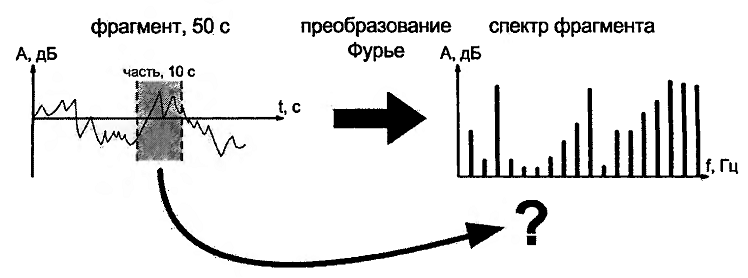
\includegraphics{pic-specter-10}
\caption{Наглядная иллюстрация действия преобразования Фурье}
\label{pic-specter-10}
\end{figure}

Таким образом, по спектру всего сигнала целиком невозможно судить о динамике его развития во времени, спектр не предоставляет информацию о том, в какой именно момент происходили те или иные изменения сигнала.

Есть еще одна причина, по которой применение блочного спектрального анализа на практике просто необходимо, а именно~--- практически невозможно подвергать спектральному анализу цельный дискретный звуковой сигнал большой продолжительности, поскольку процедура спектрального разложения (ДПФ, БПФ) такого сигнала может оказаться чрезмерно ресурсоемкой.

Итак, чтобы иметь представление об изменении спектра во времени, аудиосигнал необходимо анализировать не целиком, а по частям (говорят - "<блоками"> или "<окнами">). На рис. \ref{pic-specter-11} представлены звуковой сигнал с условной продолжительностью звучания секунд и для примера~--- три возможных способа разделения его на блоки для проведения спектрального анализа по частям.

\begin{figure}[h]
\centering
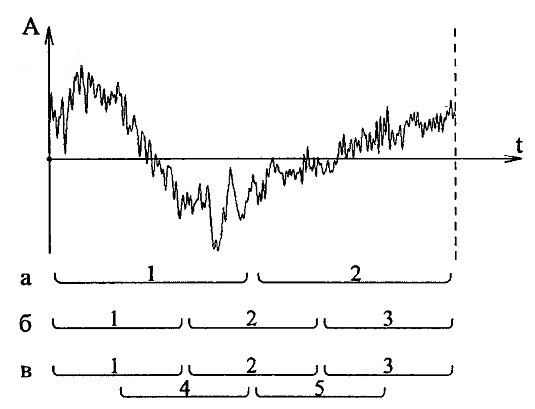
\includegraphics{pic-specter-11}
\caption{Несколько способов разделения аудиосигнала на блоки}
\label{pic-specter-11}
\end{figure}

По первому способу (вариант \(а\)) предлагается разделить сигнал пополам и проанализировать его в два приема. Два полученных спектра позволят нам понять, какие частотные составляющие присутствовали в первые \(N\).
секунд звучания, а какие~--- в оставшиеся \(N/2\) секунды. Если такого временного разрешения недостаточно, то анализ сигнала можно провести в несколько приемов, разделив его на три
(вариант \(б\)) или больше частей. Казалось бы, что для получения полной динамической спектральной картины с хорошим временным разрешением и с возможностью подробного слежения за динамикой развития спектра сигнала во времени исследуемый сигнал нужно делить на большое число коротких отрезков и рассчитывать спектр для каждого из них. Это рассуждение, в общем-то, справедливо, но имеется одна тонкость, которую нельзя не учитывать. Ведь чем короче раскладываемый в спектр участок сигнала, тем меньше информации о спектре он несет. Иначе говоря, чем более короткий участок сигнала подвергается анализу, тем менее информативный спектр получается в результате. Проанализировав сигнал целиком, мы
можем получить детальную спектральную картину, несущую максимально четкую информацию о частотных составляющих, минимально разнящихся по частоте; проанализировав же лишь небольшой отрезок сигнала, мы получаем огрубленный спектр низкого разрешения, несущий лишь приблизительную информацию об основных, наиболее выделяющихся частотных составляющих.

В итоге при проведении блочного спектрального анализа мы сталкиваемся с проблемой, решение которой строго индивидуально для каждого конкретного случая. Стремясь получить высокое временное разрешение с тем, чтобы суметь распознать более детально изменения спектра сигнала в динамике, мы вынужденно сужаем анализируемый фрагмент (блок), тем самым упрощаем его частотный спектр и теряем в частотном разрешении. Наоборот, стремясь получить как можно более детальный частотный спектр, приходится жертвовать временным разрешением, т.е. увеличивать (удлинять) анализируемый фрагмент. Эта дилемма называется
{\itshape принципом неопределенности спектрального анализа}.

\subsection{Звуки различных источников}
Рассмотрим обобщенные результаты гармонического и спектрального анализов наиболее часто встречающихся сложных звуковых сигналов, издаваемых различными источниками.
\paragraph{Человеческий голос}
Источником человеческого голоса, точнее~--- основной частоты голоса, являются голосовые связки. Звучание голоса представляется в виде сложного периодического сигнала приблизительно пилообразной формы (рис. \ref{pic-soundkind-01}).

\begin{figure}[h]
\centering
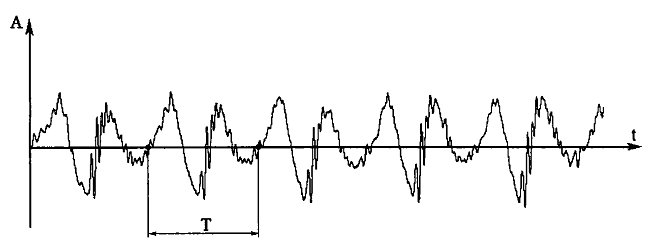
\includegraphics{pic-soundkind-01}
\caption{Сигналограмма звука "и"}
\label{pic-soundkind-01}
\end{figure}

Низшая (основная) частота в общем спектре частот у отдельных людей может составлять от 70 до 400 Гц (т.е. в одну секунду могут укладываться от 70 до 400 наибольших (основных) периодов \(T\), в связи с чем основные частоты различных по типу голосов лежат в таких пределах:
\begin{itemize}
  \item для баса: от 70 до 400 Гц;
  \item для баритона: от 110 до 440 Гц;
  \item для тенора: от 130 до 590 Гц;
  \item для контральто: от 175 до 780 Гц;
  \item для меццо-тинто: от 220 до 1050 Гц;
  \item для сопрано: от 350 до 1320 Гц.
\end{itemize}

Таким образом, можно с определенной долей вероятности говорить о нижней и верхней границах частоты основной гармонической составляющей голоса человека. При формировании звуков речи и пения, осуществляемом системой природных резонаторов речевого аппарата, подчеркиваются те или иные группы близлежащих частот их гармонического спектра (спектральные максимумы). Таких спектральных максимумов в звуке может быть четыре и больше, однако распознавание каждого звука связано с одним или двумя первыми усиленными участками спектра, которые называются {\itshape формантами}.

На рис. \ref{pic-soundkind-02} показано частотное размещение формантных областей некоторых звуков.

\begin{figure}[h]
\centering
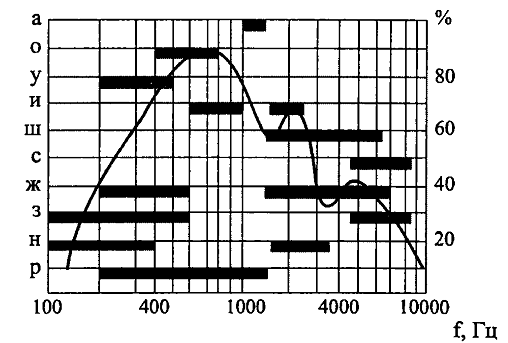
\includegraphics{pic-soundkind-02}
\caption{Частотное размещение формантных областей}
\label{pic-soundkind-02}
\end{figure}

Кривая на этом графике показывает относительное содержание формант (в процентах) в различных областях частотного диапазона. Наибольшее число формант расположено в области частот от 100 Гц до 8 кГц. Для гласных звуков характерны форманты с дискретным спектром (т.е. с явно выраженными пиками, всплесками
частот); для согласных, особенно глухих, таких как "<с">, "<ш"> и "<х">, характерны форманты со сплошным спектром. Полный спектр речевого сигнала образуется из основных тонов вместе с гармоническими составляющими, а также с формантными и неформантными областями.

Существуют специальные устройства, методы и алгоритмы, предназначенные для распознавания человеческой речи, а также идентификации человека по голосу.

\paragraph{Музыкальные инструменты}
Кратко охарактеризуем звуки, издаваемые струнными, духовыми и ударными
инструментами.

{\itshape Струнные инструменты}. Эти инструменты представляют собой акустические системы, в которых звукообразующими элементами являются туго натянутые струны, а резонаторами~--- деки и объем корпуса инструмента.

По способу извлечения звука струнные инструменты делятся на смычковые, щипковые и ударные.

К распространенным {\itshape смычковым инструментам} относятся, например, скрипка и виолончель. Максимальный уровень звукового сигнала этих инструментов не превышает 75 дБ. При возбуждении смычком струн создаются пилообразные колебания с почти постоянной амплитудой. Воздействие резонатора
сказывается в нескольких частотных областях; эти формантные области для скрипки лежат вблизи частот 400 и 800 Гц, в полосах от 2000 до 2600 Гц и от 3000 до 4000 Гц. По мере смещения главной форманты к частоте 4000 Гц качество звучания скрипки возрастает до максимума за счет подключения к главной форманте большого числа высших гармоник, с чем и связано богатство тембра, певучесть и звучность этого инструмента. При сравнении спектральных огибающих звучания струн скрипки и виолончели обнаруживается, что последние из них более плавные ("спокойные"). Однако и они имеют формантные выбросы в областях час-
тот от 250 до 300, от 400 до 500 Гц, и в области 1500 Гц.

{\itshape Щипковые инструменты} делят на две группы: грифовые и безгрифовые. К грифовой группе относятся, например, гитара, балалайка и т.д. Каждый из этих инструментов в зажатом состоянии создает ряд основных тонов, а все струны вместе обеспечивают достаточно широкий частотный диапазон. Ко второй группе относятся инструменты, струны которых не изменяются по длине в процессе игры. Это могут быть арфа, цитра и пр. Струны всех этих инструментов при возбуждении их щипком совершают собственные затухающие колебания. Для гитары общий частотный диапазон с обертонами имеет границы приблизительно от 70 Гц до 9 кГц, причем число формант, расположенных в области низких и средних частот, невелико. Основная форманта совпадает с резонансной частотой объема воздуха в корпусе. Различия в характере щипка (пучками пальцев, ногтями или медиатором) приводят к изменению частотного состава звучания. Например, при щипке с помощью ногтей или медиатора атака получается более жесткой, а звук приобретает дополнительное число гармонических составляющих. Динамический диапазон щипковых инструментов составляет порядка 20 дБ.

К {\itshape струнным ударным инструментам} относят фортепиано. Этот инструмент для создания широкого звукоряда имеет большое количество струн. Динамический диапазон равен приблизительно 45-50 дБ. Фортепиано позволяет извлекать 88 основных тонов. Самый низкий из них имеет частоту 27,5 Гц (нота "ля" субконтроктавы). Частоты всех последующих звуков увеличиваются в 1,059 (на полтона4) или в 1,122 (на тон) раза. Поэтому самый высокий из основных звуков имеет частоту 4186 Гц (нота "до" пятой октавы). Частоты и амплитуды гармонических составляющих, так же как и основных тонов, зависят от материала и размеров струн, силы их натяжения, места, длительности и силы удара молоточков по струне. Наибольшее число этих составляющих сосредоточивается в области низких частот и усиливается резонатором, особенно в пределах от 100 до 1200 Гц. Для фортепиано очень большое значение имеют временные процессы. Нарастание уровня звука при ударе молоточком по струне и почти сразу же следующее за ним затухание влияют на изменение частотного состава звучания. Так, короткое время нарастания, равное примерно 10 мс для высокочастотных и 20 мс для низкочастотных сигналов, обеспечивает большую четкость и "разделение"
 отдельных тонов. Длительный процесс затухания делает звучание фортепиано близким по мелодичности
к стационарному звучанию скрипки.

{\itshape Духовые инструменты}. В духовых инструментах звукообразующим элементом является объем воздуха, заключенного в трубе и совершающего колебания под воздействием воздушной струи, вдуваемой через отверстие. Усиление или ослабление потока вдуваемого воздуха соответственно повышает или понижает частоту колебаний. В тромбонах изменение частоты достигается также путем изменения мензуры, т.е. отношения длины потока воздуха в трубе к ее диаметру. Различают следующие духовые инструменты: дульцевые, язычковые и язычковые с амбушюром (с мундштуком).

В дульцевых инструментах возбуждение звуковых колебаний происходит при ударе вдуваемого потока воздуха о края отверстия, имеющегося в трубе. К таким инструментам относятся флейты, органные трубы и т.д. Основные тона звукоряда большой флейты лежат в пределах от 286 до 1200 Гц, а флейты-пикколо~--- в пределах от 576 до 2500 Гц. Низкочастотные трубы органа создают звучания очень низкой частоты, начиная с 16 Гц. Спектр их не очень богат.

В язычковых инструментах звук возбуждается благодаря периодическому колебанию одной-двух пластинок, перекрывающих отверстие для вдувания воздуха. К инструментам такого типа можно отнести, например, кларнет, гобой и фагот. Полный частотный спектр фагота укладывается в пределах от 60 до 2500 Гц. Сильные форманты для этого инструмента располагаются у частот 500 и 1500 Гц.

К числу язычковых инструментов с амбушюром относятся труба, валторна, тромбон. Чашкообразный мундштук подчеркивает высокочастотные составляющие звуков трубы и тромбона. Воронкообразный мундштук валторны, наоборот, ослабляет составляющие на высоких частотах. В среднем эти инструменты имеют динамический диапазон 40 дБ.

{\itshape Ударные инструменты}. В инструментах ударного типа в качестве звукообразующего элемента используются бруски, пластины или мембраны, а их возбуждение осуществляется ударом пластин друг о друга (тарелки) или ударом колотушки (ксилофон, челеста). Очень тонкие, гибкие пластины натягиваются на жесткие каркасы (барабаны, литавры).

Ударные инструменты пластинчатого типа делят на инструменты с определенной частотой колебаний (ксилофон, челеста) и с неопределенной частотой колебаний (тарелки и пр.). В последних одиночный звук имеет сложную непериодическую структуру и как следствие~--- большое число негармонических составляющих.
Динамический диапазон зависит от материала, из которого изготовлены пластины: для тарелок~--- около 60 дБ, для ксилофона и металлофона~--- 25-30 дБ, для челесты~--- 20 дБ. Основные звуки таких инструментов укладываются в диапазон частот от 300 до 4500 Гц.

Мембранные инструменты отличаются большой мощностью и широким диапазоном звучания. Яркими представителями инструментов мембранного типа являются литавры и барабаны. Динамический диапазон литавр равен приблизительно 80 дБ, большого и малого барабанов~--- 70 дБ. Барабаны имеют звуковые колебания с большим количеством негармонических составляющих. Их частотные диапазоны лежат в пределах от 50 до 6000 Гц. Длительность послезвучия этих инструментов зависит от массы и силы натяжения мембраны и достигает нескольких секунд.

\section*{Литература}
\begin{enumerate}
\item Радзишевский, А.Ю. \emph{Основы аналогового и цифрового звука}.~--- М. : Издательский дом "<Вильямс">, 2006.~--- 288с.
\item \emph{Акустика: Учебник для ВУЗов}. Ш.Я.Вахитов, Ю.А. Ковалгин, А.А.Фадеев, Ю.П.Щевьев; Под ред. профессора Ю.А. Ковалгина.~--- М. : Горячая линия~--Телеком, 2009.~--- 600с.
\item \emph{Акустика: Справочник}. А.П. Ефимов, А.В. Никонов, М.А. Сапожков, В.И. Шоров; Под ред. М.А. Сапожкова.~--- 2-е изд., перераб. и доп.~--- М.: Радио и связь, 1989.~--- 336с.
\end{enumerate}

\end{document} 